\chapter{Foundations: causal inference}\label{sec:3}
In this chapter, I give a concise introduction to the basic notions and methods of causal inference. Since this branch of statistics is quickly growing into a large field, the discussion is focused on leading the reader towards an understanding of the theory behind the methods I am developing. This implies that the exposition will only consider methods which are applicable to discrete data, and disregard the many methods which are being developed and improved for continuous observations.

\section{Philosophical and theoretical foundations}\label{sec:3:1}
This section starts with a look at the very basic intuitions and established principles of the field. After some general considerations about the well-known issues in linking correlation to causation, we motivate the need for causal thinking even in the absence of experiments, and turn to the central idea of using nature as an experimenter.

I then introduce the crucial notion of conditional independence between variables, which roughly amounts to a criterion for deciding whether the connection between two variables can be explained away by considering the possibility of mediating other variables. For instance, there probably is a measurable correlation between the occurrence of hats and trousers as pieces on the clothing of humans, which might disappear when we condition on gender. The gender of the body suffices to predict how likely we are able to find a hat or trousers on it, and there is no direct connection in the sense that putting a hat on one's head would cause one to also put on trousers, or the other way around.

Sets of conditional independence statements over a set of variables identify a graphical model over these variables, which is a decomposition of the joint distribution into factors given by a neighborhood relation in a graph. I will present some mathematical notions which were developed to make this relationship more precise, allowing us to exploit it for inferring graphical models from data.

Crucially, the Bayesian networks we can infer from data can be given a causal interpretation. If we see such a structure not as a compact way to model and a convenient handle for calculating a joint distribution, but as representing the actual information flow between the variables, we can interpret each directed edge in a graphical model as expressing a causal influence from the starting variable to the variable the edge goes into. Based on this initial idea, one can build an entire theory of intervention, allowing us to predict what would happen if one of the variables was given a certain fixed value by manipulation, as in an experiment. \cite{pearl2009} summarizes a wealth of previous work in this direction.

In this book, the emphasis is not on the philosophical issues about causality which the intervention calculus touches upon, but on exploring the idea of defining causal graphs over languages, and interpreting the directed arcs as indicating how languages influenced each other. In this section, we start with some general considerations about causality, and the way complex probability distributions are represented by directed graphs in the Bayesian network paradigm. I then introduce the central idea behind causal inference, i.e.\ giving a causal interpretation to the efficient representations generated by Bayesian network inference. The mathematical details are then the subject of the next section.

\subsection{Correlation and causation}
There are three major reasons why the common warning that correlation is not causation is true. The first is that correlation does not tell us the direction of causality. Secondly and even more importantly, for any observed correlation of two variables it is always possible (even likely) that there is a \textit{\isi{hidden common cause}} or \textit{\isi{confounder}} which influences both variables. In this case, the correlation is not due to a true causal connection which would link the two variables directly, but due to \textit{confounding bias}. The third problem is \textit{\isi{selection bias}}, a second type of bias which can cause non-causal correlations, and can occur whenever two observed variables have an influence on the sampling process. Selection bias is a very difficult problem for clinical studies, because participation in the study frequently depends on both the strength of symptoms and the availability of treatment, which can create a spurious impression for some treatment to have an effect on the symptoms.

To illustrate the general applicability of the causal inference framework, I will work with two running examples throughout this chapter. For our more classical example with actual statistical variables, take the variable $R$ to mean the average room temperature during the winter months, which we can measure in any household of an entire country. Let $O$ be the average outside temperature in the respective city during the same timeframe, $H$ the heating costs per square meter for the household, and $I$ some measure of the household income. In a wealthy welfare state where virtually everyone can afford as much heating as they want, I would assume the average room temperature $R$ to only be based on personal preferences $P$, and hence independent of both the outside temperature $O$ and household income $I$. Since people will try to maintain their desired room temperature $R$ by influencing $H$, there will obviously be a negative correlation between $H$ and $O$. On some level, this does mean that lower outside temperatures cause heating costs to increase, but this is only the case because people are trying to keep $R$ constant, i.e.\ the causality is mediated by the room temperature, on which both the amount of heating and the outside temperature have a causal effect.

To give an example of selection bias, assume a politician wanted to argue for a policy that prevents poor people from spending too much money on heating. In anonymized data provided by a consumer counseling service, there does indeed turn out be a strong correlation between $I$ and $H$, seemingly supporting the policy. The problem is that this is very likely a spurious correlation due to selection bias, because low-income households with high heating costs (e.g. due to high $P$) are much more likely to get counseling, and thereby becoming part of the study, than other households.

In lexical flow inference, I will model language varieties as variables which influence each other's lexica. The second running example in this chapter serves to establish and illustrate this view, taking the first steps to an abstract understanding of the approach before we turn to the data needed for an implementation in \chapref{sec:4}, and the actual mathematical details in \chapref{sec:6}. I will often be deliberately vague in this chapter when I write about computing the correlation between languages, or explaining the dependence between two languages based on a third one, in order to demonstrate how general the reasoning patterns are, and that they would apply to many ways of modeling language varieties as mathematical objects. The algorithms in Chapters 6 and 7 will be based on one particular way of fleshing out these reasoning patterns in terms of shared cognates, but the general reasoning patterns could just as well be applied to typological variables, measures on parallel texts, and many other mathematical 
models of language.

\largerpage
Generally, if we have some measure of determining whether two languages are related or not, we can frame this relation in terms of independence. For instance, the languages \ili{Japanese} (\textit{jpn}) and \ili{Icelandic} (\textit{isl}) are commonly assumed to not be demonstrably related, and should therefore be independent according to any reasonable measure. On the other hand, the languages \ili{Danish} (\textit{dan}) and \ili{German} (\textit{deu}) are related, and should therefore come out as dependent. Danish and German do, in fact, have a hidden common cause, namely their latest common ancestor Proto-Germanic (\textit{PGer}). In addition, Danish includes many loanwords from German, which a good model would detect as additional correlation in addition to the amount of correlation caused by the common proto-language, and ideally, it would make it possible to determine German as the source of borrowing. We would thus frame the Danish lexicon as being ``caused'' by the words of Proto-Germanic and German.

With this general idea in place, let us stop and consider the question to what extent we can say that the lexicon of a language is caused by the lexicon of its immediate ancestor, as well as the lexica of any donor languages. To get a more concrete picture of the actual process underlying this way of thinking, we need to move down to the level at which the process which perpetuates a language actually operates. This process boils down to the acquisition of a language by single speakers, which can effectively stretch across throughout much of their lifetimes. When a child acquires words, the languages of the parents or other close relatives will likely be the source of these words. During later development, speakers might be exposed to additional languages (such as a dominant state language) at school, at the workplace, or while traveling, which adds additional speakers to the list of causes for their lexicon. But even within the same language community, speakers will continually acquire new words which they hear from other humans that they are in contact with. On the most elementary level, the language of an individual speaker can thus with some justification be said to be caused by the languages of other speakers. The causal metaphors becomes more problematic if we lift it to the level of entire languages, summarizing thousands or millions of individual speaker histories to the level where we speak of Proto-Germanic causing German, even if not directly. It would even be wrong to say that the language of one generation is the main cause of the language of the next, because on the level of a population, a generation is just as artificial a category as the language stages I mentioned at the end of the previous chapter. Still, with the disconnect between our abstraction and the actual process in mind, conceiving of languages as being caused by their ancestors as well as additional donor languages will turn out to be a very fruitful metaphor.

\subsection{Causality without experiment}
At least since \cite{fisher1925}, one of the foundational works of modern statistics, the mainstream view on causality has been that it can only be determined by experiment, i.e.\ by manipulating one of the variables while observing the effect on the others. When analyzing observational data without the possibility of manipulation, the principle has been to avoid thinking in causal terms, because there was no way of giving a causal interpretation to observed correlations. This inability and prudent refusal to talk about causality has left classical statistics in a rather problematic situation. Most applied statistics is arguably motivated by causal thinking, because a prime motivation of research is to find out why things happen. For this reason, results obtained from observational data will invariably be given causal interpretations, as questionable as that may be from the statistical point of view.

A very promising and comparatively recent approach to alleviating this tension has arisen in the field of causal inference, where causal notions receive a systematic and consistent treatment with the help of graph theory. From the perspective of inference, the core idea is to see nature as an experimenter, in the sense that the random fluctuations in various variables are comparable to manipulations in experiments, even though they are not performed by humans, and certainly not under controlled conditions. For this reason, even more careful thinking is required to avoid the pitfalls which even controlled experiments suffer from. We must ensure that all the possibly relevant variables are taken into consideration, so that there are no confounders leading us to the wrong conclusions. Moreover, this view requires us to put belief into the \isi{common cause principle} (CCP), most often attributed to \citet[Ch. 19]{reichenbach1956}, where the original formulation reads as follows: ``If an improbable coincidence has occurred, there must exist a common cause''. In statistical terms, this principle implies that variables are typically not correlated by chance. Any significant correlation between two variables must be due either to a direct causal relationship (in whichever direction), or, if they are measured simultaneously, a common cause.

In our heating costs scenario, I would expect to see a correlation between $I$ and $H$, indicating that more wealthy households will have higher heating costs per square meter. It does not make sense to posit either that $I$ causes $H$ (a low wage makes it easier to keep each square meter of your house warm), or that $H$ causes $I$ (higher heating costs increase your wage), so according to the CCP there must be a common cause influencing both $I$ and $H$. After some research, we might find that rich people have a tendency to afford larger windows, which decreases their building's heat insulation and makes it more expensive to maintain the desired room temperature. We might therefore include the confounder into our model, as a variable $W$ measuring the window expanse per square meter. If we have no way of measuring this variable, it becomes a hidden confounder that we need to take care of.

For the language scenario, the CCP applies as well, because we would also expect any similarity between languages to be explainable either by chance (in case the correlation is not significant, for example), by a direct causal relationship (i.e. borrowing), or by a common cause (e.g., a common proto-language, or a common source language for shared loans). The case of an additional confounder that needs to be included into our theory may occur in the case of a common substrate layer.

\subsection{Conditional independence}
Two statistical variables $X$ and $Y$ are said to be \textit{independent}\is{independence}, which we write as $(X \independent Y)$, iff $p(x,y)=p(x)p(y)$ for all values $x$ of $X$ and $y$ of $Y$. Intuitively, independence means that we do not know any more about the value of $Y$ if given the value of $X$, and vice versa.

In our example scenario, we assumed the room temperature $R$ to be independent of the household income $I$. The definition implies that if we know the distribution of room temperatures and the distribution of household incomes, we can predict the joint probability $p(R,I)$ for any given values of $R$ and $I$. Knowing the average room temperature does not allow us to make a more educated guess about whether we are dealing with a high-income household, and vice versa. In contrast, we said that the outside temperature and the heating costs are not independent. Knowing the outside temperature will change our expectations about the heating costs, and vice versa.

There are many ways in which independence could be defined over languages. If two languages like \ili{Japanese} and \ili{Icelandic} are independent, the definition implies that if we know, for example, the word for some animal in Japanese, this will not help us in any way to predict how that animal might be called in Icelandic (\iso{jpn} $\independent$ \iso{isl}). In contrast, if we know that a snake is called \textit{slange} in \ili{Danish}, this will allow us to make a more educated guess about the \ili{German} word. Such an educated guess might be successful in some cases (German \textit{Schlange} `snake') and less successful in others (Danish \textit{ræv} vs. German \textit{Fuchs} `fox'), but knowledge of the one language helps us to predict the word in the other languages in enough cases to be statistically relevant (\iso{dan} $\notindep$ \iso{deu}). 

Moving one step further, the central notion for causal inference is the \textit{conditional independence} of a pair of (sets of) variables given a set of other variables. If two variables $X$ and $Y$ are dependent, but conditionally independent given a set of variables $Z$, we say that the dependence disappears when \textit{conditioning on} $Z$. Intuitively, if we know the values of the variables in $Z$, knowing the value of $X$ will not tell us anything new about the value of $Y$, and knowing $Y$ will not add to our knowledge about $X$.

\newpage 
For the formal definition, let $p$ be a joint probability function over a finite set $V$ of variables. For any sets $X,Y,Z \subseteq V$, we say that $X$ and $Y$ are conditionally independent\is{conditional independence} given $Z$ [in symbols: $(X \independent Y\ |\ Z)$] if $p(x|y,z) = p(x|z)$ whenever $p(y,z) > 0$.

In the heating example, we will certainly observe a dependence $(P \notindep R)$ between the temperature preference $P$ and the room temperature $R$. However, it is certainly not the case that the room temperature will drop just because we want it to do so, and a rising temperature in the bedroom will only increase our discomfort, but not the temperature at which we would want to sleep. Instead, the process connecting these two variables is mediated by the heating costs $H$, and we are going to have $(P \independent R\ |\ H)$ because if we are not allowed to manipulate the heating, our preferences will not have any impact on the room temperature any longer.

Conditional independence relations hold between many types of knowledge we might have about languages as well. For instance, \ili{Swedish} (\textit{swe}) is more closely related to \ili{Danish} than \ili{German} is, which is why on average, additional knowledge of German will not help us to understand a Swedish word if we already understand the Danish one $(swe \independent deu\ |\ dan)$. To illustrate, take the words for `bird' (\textit{fågel/fugl/Vogel}), where German would have helped almost as much as Danish, and the words for `ant' (\textit{myra/myre/Ameise}), where Danish is much closer to Swedish. The latter example also shows why we would likely get $(swe \notindep dan\ |\ deu)$ from any useful criterion of conditional independence.

The conditional independence relation $(X \independent Y\ |\ Z)$ has a number of interesting properties, most of which should be intuitively obvious. For instance, it satisfies \textit{symmetry}\is{symmetry property} in the sense that $(X \independent Y\ |\ Z)$ implies $(Y \independent X\ |\ Z)$, which we can interpret to mean that if $X$ does not tell us anything about $Y$, neither will $Y$ provide us with any information about $X$. This is a very natural assumption for languages as well, since language relatedness is a symmetric relation. 

It also has the \textit{decomposition} property\is{decomposition property} in the sense that jointly irrelevant pieces of information do not become relevant when considered separately, i.e.\ $(X \independent YW\ |\ Z) \Rightarrow (X \independent Y\ |\ Z)$. For instance, given that the knowledge of both a person's income and his or her temperature preferences does not allow us to draw any conclusions about the climate, it makes sense to assume that neither will income or preference data alone. To understand why the decomposition property holds for languages as well, consider the situation where two groups of languages do not share any features that are not explainable by a third set of languages. If this is the case, this third set will also explain all the overlap between individual languages from the two groups. For instance, if we have established that Proto-Indo-European can be used to explain all similarities between Indo-Aryan\il{Indo-Aryan languages} and \ili{Germanic languages} $(IndoAryan \independent 
Germanic\ |\ PIE)$, we can conclude that it will also explain the (fewer) similarities between individual language pairs such as \ili{Sanskrit} and \ili{German} $(san \independent deu\ |\ PIE)$, or \ili{Pali} and \ili{English} $(pli \independent eng\ |\ PIE)$.

Another property is \textit{weak union}\is{weak union property}, which states that an irrelevant piece of information $Y$ will not suddenly become relevant if we learn another irrelevant piece of information $W$, or $(X \independent YW\ |\ Z) \Rightarrow (X \independent Y\ |\ ZW)$. In the heating cost example, neither the household income nor the outside temperature allow us to say anything about the room temperature, and we would be very surprised if, say, a correlation between the two temperatures would appear once we look at rich households only. For groups of languages whose similarities are explained by a third language, like in the previous example situation $(IndoAryan \independent Germanic\ |\ PIE)$, we would not expect one of the languages from one group (say, \ili{Gothic}) to provide additional information that makes the remainder of the group appear more similar to Indo-Aryan\il{Indo-Aryan languages}, i.e. we would also expect $(IndoAryan \independent NWGermanic\ |\ PIE, Gothic)$. The weak union property thus mirrors the informativeness of languages in historical linguistics, where relevant (i.e. non-random) similarities will always become clearer if additional languages are taken into account.

Conversely, a \textit{contraction} property\is{contraction property} also holds, stating that information $W$ that is irrelevant after learning another piece of irrelevant information $Y$, must have been irrelevant all along: $(X \independent Y\ |\ Z)  \wedge (X \independent W\ |\ ZY) \Rightarrow (X \independent YW\ |\ Z)$. In the heating costs example, we know that the outside temperature $O$ is not connected in any way to household income $I$. Assume that in two separate studies of richer and poorer people, no connection between people's preferences $P$ and the outside temperature $O$ was found, i.e.\ it was established that $(P \independent O\ |\ I)$. In this situation, it would appear nonsensical if it turned out that in the overall population, we had $(P \notindep O)$. Similarly, considering the relationships between branches of Indo-European\il{Indo-European languages}, if we used Iranian\il{Iranian languages} evidence to explain the similarities between Slavic\il{Slavic languages} and \ili{Armenian} $(
Slavic \independent Armenian\ |\ PIE, Iranian)$, but also found that Slavic and Iranian are independent branches that did not remain in similarity-inducing contact after the split-up of Proto-Indo-European $(Slavic \independent Iranian\ |\ PIE)$, we know that we would have needed Iranian to split Slavic from Armenian. On the other hand, contraction does not exclude the possibility that $(Iranian \notindep Armenian\ |\ PIE)$, which we would actually not be surprised to find given the considerable influence of Iranian languages on Armenian.

Finally, there is an \textit{intersection} property\is{intersection property} stating that if given some other knowledge $Z$, two sets of variables are mutually irrelevant to a set of variables $X$, neither of them will be relevant to $X$ in isolation (nor jointly, by decomposition): $(X \independent W\ |\ ZY)  \wedge (X \independent Y\ |\ ZW) \Rightarrow (X \independent YW\ |\ Z)$. Expanding on the heating cost example to get an instance of this reasoning pattern, let us introduce the latitude $L$ into the picture. Obviously $L$ is going to influence $O$. Moreover, assume that due to historical scarcity of heating materials, people in climates with lower $O$ have developed a culture that reduces the window size $W$. In this situation, where both $(L \independent R\ |\ O, W)$ and $(L \independent W\ |\ O, R)$ hold, we would not expect to find either $(L \notindep R\ |\ O)$ or $(L \notindep W\ |\ O)$, because the average outside temperature should already provide all the necessary explanation for the connection 
between latitude and window size. To also motivate the intersection property among sets of languages, we will consider a likely configuration of conditional independence statements involving \ili{Irish} (\textit{gle}), \ili{Icelandic} (\textit{isl}), and \ili{Spanish} (\textit{spa}). Since these three languages come from separate branches of Indo-European, and have not been in contact since PIE split up, we would expect $(gle \independent isl\ |\ PIE, spa)$ and $(gle \independent spa\ |\ PIE, isl)$ to hold in the absence of selection bias. These constraints say that provided with background information about the common Indo-European elements, Icelandic does not tell us anything new about Irish if we already know Spanish, but neither does Spanish if we already know Icelandic. In this situation, it would be nonsensical to assume that both languages together would provide any relevant information about Icelandic, which is mirrored by the intersection property telling us that $(gle \independent isl, spa\ |\ PIE)
$. To understand why this reasoning pattern is only valid if the irrelevance is mutual, consider the same situation with \ili{Dutch} (\textit{nld}) and English instead of Icelandic and Spanish. The situation for Dutch is similar to the one for Icelandic, so that we will have $(gle \independent nld\ |\ PIE, eng)$, but the reverse does not hold any more, because English and Irish have been in contact $(gle \notindep eng\ |\ PIE, nld)$.  Here it makes sense that the reasoning pattern does not apply, because otherwise we had $(gle \independent nld, eng\ |\ PIE)$, which would imply the wrong statement $(gle \independent eng\ |\ PIE)$ by decomposition.

After stating the different properties of conditional independence, and understanding that they represent very general reasoning patterns that make sense in many domains, we can now take the decisive step connecting conditional independence constraints to graphs. If we picture the different variables as nodes, and the edges as communication channels which allow the transfer of information in both directions, we find that the conditional independence relation can be assigned a straightforward interpretation in terms of paths in a graph. If we define $(X \independent Y\ |\ Z)$ as meaning that every path from a node in $X$ to a node in $Y$ will be blocked by some node in $Z$, the relation has the same five properties, which are therefore called the \textit{graphoid axioms}\is{graphoid axioms}. Together, they have been found to characterize informational relevance very well in many different contexts, and the examples may already have convinced the reader how close the correspondence in fact is. Conditional 
independence relationships will give us testable elementary statements which we can use to construct graphs over languages, such as the one in \figref{fig:langGraph}, which will become our running example to illustrate my view on lexical flow networks. In this much simplified picture of the interactions as reconstructed by linguists, the edges represent information flow, and more specifically, the flow of lexical material, between various historical stages of the three major languages of East Asia. For instance, the theory represented by the graph states that the information flow from \ili{Old Chinese} to \ili{Old Japanese} was mediated either by \ili{Middle Chinese} or \ili{Old Korean}, whereas Middle Chinese directly influenced it. In the next section, we will establish a systematic correspondence of such path constraints with conditional (in)dependence statements such as, in this case, $(OC \independent OJ\ |\ OK, MC)$ and $(MC \notindep OJ\ |\ OK, OC)$.

\begin{figure}
 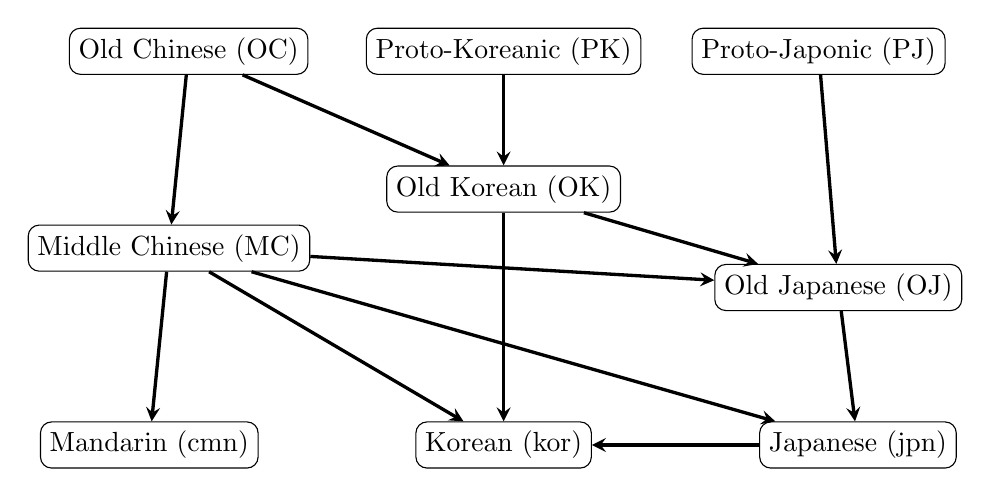
\begin{tikzpicture}
  [scale=.5,auto=left,every node/.style={shape=rectangle, rounded corners,
    draw, align=center}]
  \node (OC) at (1,11) {Old Chinese (OC)};
  \node (PK) at (9,11) {Proto-Koreanic (PK)};
  \node (PJ) at (17,11) {Proto-Japonic (PJ)};
  \node (MC) at (0.5,6) {Middle Chinese (MC)};
  \node (OK) at (9,7.5) {Old Korean (OK)};
  \node (OJ) at (17.5,5) {Old Japanese (OJ)};
  \node (cmn) at (0,1) {Mandarin (cmn)};
  \node (kor) at (9,1) {Korean (kor)};
  \node (jpn) at (18,1) {Japanese (jpn)};
  \begin{scope}[very thick, -stealth]
  \foreach \from/\to in {OC/MC,MC/cmn,PJ/OJ,MC/OJ,MC/jpn,MC/kor,OC/OK,PK/OK,OK/kor,OJ/jpn, OK/OJ,jpn/kor}
     \draw (\from) -> (\to);
  \end{scope}
  \end{tikzpicture}
 \caption{Example graph over (selected) languages of East Asia}
\label{fig:langGraph}
\end{figure}


As a final remark about conditional independence, it is worth emphasizing that conditioning on additional variables can not only remove dependencies, but it can also induce dependencies between otherwise independent variables. As stated earlier for our heating costs example, we are likely to observe an independence $(R \independent O)$ if we do not condition on anything else. However, this is only the case because people will regulate the heating to ensure a constant $R$. But any fixed investment $H$ into heating will be more or less effective at different outside temperatures. For fixed $H$, room temperature will therefore begin to depend on the outside temperature, so that we have a conditional dependence $(R \notindep O\ |\ H)$, whereas we had $(R \independent O)$. This is also the pattern underlying selection bias, which can be treated in the framework of conditional independence relations by introducing a hidden selection variable $S$, and assuming that the data are actually from the conditional 
distribution given $S$. This effectively turns every statement of the form $(X \notindep Y)$ into an underlying $(X \notindep Y\ |\ S)$, which does not contradict $(X \independent Y)$ in the underlying truth. 

Selection bias is a frequent problem in the application of statistical arguments within historical linguistics. For any linguist trying to prove that two groups of languages are related, it is difficult to avoid a natural tendency to filter the material in some way, e.g. by focusing on certain parts of the vocabulary that seem more promising. This becomes a problem as soon as statistical testing comes into play, where bias-free sampling is essential for estimating the amount of similarity that we would expect by chance, and therefore correctly determining the significance level. To illustrate that selection bias can also have an impact on purely data-driven approaches, assume that we want to assess by large-scale vocabulary comparison whether there is a hidden common ancestor between \ili{Basque} (\textit{eus}) and \ili{Albanian} (\textit{sqi}), such as a common Old European substrate. In a balanced sample of our vocabulary, we would very likely find $(eus \independent sqi)$. Now assume that we want to build the analysis on parallel word lists which include the oldest attested languages of Europe, such as \ili{Gothic} (\textit{got}). If the compiler of these word lists had any tendency to tune the selection of concepts towards those for which a Gothic word is known, e.g. in order to create a more fully populated table, the nature of the only available longer Gothic text (a Bible translation) will induce a selection bias. Both Basque and Albanian are heavily influenced in their religious vocabulary by \ili{Latin} and \ili{Romance languages}, which could easily lead to a statistically significant similarity on the word list $(eus \notindep sqi\ |\ got)$, even though we only considered data for the two languages, and might erroneously conclude that $(eus \notindep sqi)$. The same could happen in corpus-based approaches that rely on religious texts such as Bible translations, which are quite frequently the only available written records especially of smaller languages that do not have an indigenous writing tradition.

\largerpage[-1]
\subsection{Bayesian networks}
The more variables we consider, the more difficult it becomes to estimate and represent their joint distribution. However, if factorizations of the joint distribution function are possible, they can be used to build a directed acyclic graph (DAG) where each node contains the conditional probability distribution of one variable given a set of parent variables. The resulting \textit{Bayesian networks}\is{Bayesian network} provide a very compact way of representing joint distributions of many variables, and lend themselves very well to a range of important inference tasks. \cite{pearl1988} is the classical book on Bayesian networks, which explains many of the basic notions and issues in a very detailed and readable fashion, including the motivation of the following definitions.

Let $p(v)$ be the joint probability distribution on an ordered set $V = \{X_1,\dots,X_n\}$ of variables. A set $PA_j \subset V$ is said to be the \textit{Markovian parents} of a variable $X_j \in V$ if it is a minimal set of predecessors of $X_j$ that renders $X_j$ independent of all its other predecessors. In our East Asian example, $\{OJ,OC\}$ is not the set of Markovian parents of \ili{Japanese}, because according to the graph, this set does not explain all the overlap between \ili{Middle Chinese} and Japanese. Adding Middle Chinese to the set will still not give us the Markovian parents of Japanese, because the subset $\{MC,OJ\}$ already covers all paths from any other language into Japanese, and \ili{Old Chinese} is not a Markovian parent, because it is screened off by the other two languages in the set $\{MC,OJ\}$, which is therefore the set of Markovian parents of Japanese. Note that the situation could be different if we had chosen to model, say, Middle Japanese in addition, which would replace Old 
Japanese in the set of Markovian parents.

If a probability function $p$ admits the factorization $p(x_1,\dots,x_n) = \prod_i p(x_i\ |\ pa_i)$ relative to a DAG $G$, we say that $p$ and $G$ are \textit{(Markov) compatible}. In words, each variable must be independent of its non-descendants in the graph if the state of its Markovian parents is known. We say that a joint distribution fulfills the \textit{Markov condition}\is{Markov condition} if there is some graph to which it is compatible. As we have seen, the graph is mirrored by a factorization of the joint probability distribution, which can be used to compactly represent and efficiently perform calculations on joint and marginal probabilities.

Later textbooks such as \cite{koller_friedman_2009} build on a much more advanced theory and two decades of practical experience in applying graphical models to many problems. However, Bayesian networks have developed into a separate field which is mainly concerned with other tasks, such as the efficient inference of marginal distributions from joint distributions encoded as networks. This newer literature might therefore serve less well to lead the viewer towards an understanding of their importance for causal reasoning, a topic which we turn to in the next section.

\subsection{Causal interpretation of {B}ayesian networks}
From a philosophical angle, it appears attractive to give a causal interpretation to Bayesian networks, taking the directed arcs in Bayesian networks to represent direct causal influence of one variable on another. \cite{pearl2009} presents a range of ideas that follow from this viewpoint. Reinterpreting Bayesian networks not as convenient representations of joint probability distributions, but as causal DAGs which actually model the causal processes that generated the data, makes it possible to predict what happens if one of the variables is manipulated from the outside. Pearl develops this idea into a full intervention calculus, providing a framework for calculating answers to counterfactual questions as they arise in jurisdiction when, for instance, responsibility for an accident needs to be decided, and which previously were notoriously difficult to grasp mathematically. As Pearl shows, his fresh view of causality also provides a handle on long-standing statistical paradoxes like Simpson's paradox, where the direction of a correlation between two variables can revert in each individual case when we consider all values of a third value separately. Using the calculus of interventions with its true manipulation operation distinct from conditioning, the seeming paradoxes instantly disappear. As Pearl shows, they only existed due to a confusion of conditioning and manipulation, two operations which the classical statistical methods could not cleanly distinguish. By giving a causal interpretation to Bayesian networks, and thinking about experiments as manipulating the network, we gain a mathematical language for speaking about causality.

Stepping back from predicting the consequences of manipulation, the conditional independence relations we can extract from observational data can be exploited systematically to infer parts of the process which generated the data. This algorithmic side of causal analysis was further developed by \cite{spirtes_ea_2000}. Their book provides many of the technical proofs for the theory of inferred causation, and contains the first versions of several central algorithms which I will build upon in this book. It also provides a wealth of impressive examples, including a very in-depth discussion of how causal inference can be used on existing data to prove once and for all that smoking does cause lung cancer. The argument effectively destroys the tobacco industry's last line of defense, which consisted in claiming that the correlation might be due to a genetic predisposition which causes both a taste for cigarettes, and a propensity to develop lung cancer, an explanation which seems absurd, but cannot be ruled out by 
classical statistical methods.

In this book, I explore how this framework can be applied to languages. If we manage to model language graphs such as the East Asian example in \figref{fig:langGraph} as Bayesian networks, we can give a causal interpretation to the arrows, and should be able to use causal inference in order to infer the structure of the network which generated the observable data. If our observations consist of lexical data (as they do in this book), the causal graph can be interpreted as a minimal explanation of how the observed patterns could result from languages influencing each other, either by inheritance (as in the case of \ili{Old Chinese} and \ili{Middle Chinese}) or by borrowing (as in the case of \ili{Japanese} influence on \ili{Korean}). Each directed arc will represent the transmission of lexical material, and depending on how the underlying conditional independence tests are implemented, each link will correspond to a set of etymologies, detailing which words the model assumes to have been transmitted  along which path through the network.

Unfortunately, as we shall see, applying causal inference in practice to a new domain is a lot less straightforward and instantly rewarding than such examples would suggest. The proliferation of additional approximation tricks and processing steps in the literature is a tell-tale sign that one should never expect readily available implementations to yield useful results on a new problem, such as lexical flow modeling in my case. Still, most work on causal inference takes place within the confines of an almost canonical set of basic ideas and algorithmic procedures, and it is this core of the causal toolbox that I will be introducing throughout the rest of this chapter.

\section{Causal inference algorithms}\label{sec:3:2}
This section introduces the basics of \textit{causal inference} or \textit{causal discovery}, which is defined as the task to analyse a set of data (observations of three or more variables) to find a \textit{causal structure} (a partially directed acyclic graph) which mirrors the data-generating process as closely as possible. After laying out the basic assumptions and theorems which link conditional independence relations to constraints on the graph structure, I will give an overview of different approaches to testing for conditional independence, and then proceed to motivating and describing the most important causal inference algorithms. Pointers to the relevant literature will enable the reader to find proofs and more general variants of the various mathematical theorems which are needed to explain the motivation behind the algorithms, and why they work.

\subsection{Causal graphs}\label{sec:3.2.1}
I start by defining precisely the mathematical objects that I will be operating on. After defining different types of (partially) directed graphs which can be used to represent causal structures, and basic graph-theoretic notions which will be needed afterwards, I introduce the central notion of d-separation, and its generalization to ancestral graphs. Then, the main assumptions and theorems which link conditional independence relations and possible causal graphs are cited and put into context.

\subsubsection{Basic definitions}
A \isi{causal graph} $G = (V,E)$ consists of a set of nodes $V$ which represent random variables, and a set of edges $E \subset V \times V$ which will be taken to represent the causal connections between those variables. In the more general variant where the presence of hidden common causes and selection bias cannot be excluded, we have a partition $E = E_\rightarrow \cup E_\leftrightarrow \cup E_\text{---}$ into directed arcs which represent direct causal links, bidirected arcs which represent the existence of a hidden common cause for the two variables in question, and undirected arcs to represent the presence of selection bias inducing a dependence between two variables. For each of the three relation types, we will typically just write $X \text{ --- } Y$ for $(X,Y) \in E_\text{---}$, $X \rightarrow Y$ for $(X,Y) \in E_\rightarrow$, and $X \leftrightarrow Y$ for $(X,Y) \in E_\leftrightarrow$.

There is some convenient short-hand terminology which can be used to talk about the relations defined by the different edge types. For instance, the asymmetric directed arcs in $E_\rightarrow$ define the \textit{parent} relation\is{parent relation}, and in subsequent definitions I will write $pa(X) := \{Y \in V\colon (Y,X) \in E_{\rightarrow}\}$ ro refer to the set of parents of $X$.

A \textit{path}\is{path (in graph)} in a graph $G$ is a sequence $\langle X_0,\dots,X_n \rangle$ of distinct vertices $X_0,\dots,X_n$ where $(X_i,X_{i+1}) \in E$ for $0 \leq i < n$. If in addition, $(X_i,X_{i+1}) \in E_\rightarrow$ for all $0 \leq i < n$, we have a \textit{directed path}\is{directed path (in graph)} from $X_0$ to $X_n$. If there is directed path from $X$ to $Y$, or $X = Y$, $Y$ is called a \textit{descendant}\is{descendant (in graph)} of $X$, and $X$ an \textit{ancestor}\is{ancestor (in graph)} of $Y$. For the set of ancestors of any node $X \in V$, we will write $an(X)$. Applying this terminology to our example network of East Asian languages, there is a directed path from \ili{Old Chinese} to Mandarin\il{Mandarin Chinese}, but no directed path from \ili{Japanese} to Mandarin. Deviating from the standard terminology in historical linguistics, where every language has a single ancestor, and the recipient language of a layer of borrowings is not called a descendant of the donor language, in 
graph terminology Old Chinese is an ancestor of both Mandarin and Japanese, whereas Japanese is a descendant of both \ili{Old Japanese} and \ili{Middle Chinese}.

\newpage 
A \textit{\isi{directed cycle}} pattern exists whenever we have a directed path from $X$ to $Y$, but also a link $Y \rightarrow X$, allowing us to get back to the beginning of the path. Similarly, an \textit{\isi{almost directed cycle}} consists of a directed path $\langle X,\dots,Y \rangle$ and a bidirected arc $Y \leftrightarrow X$. In our East Asian language network, we do not have a directed cycle, and due to their temporal nature such cycles will not typically occur in language networks, unless we collapse different stages of three languages between which contacts in all directions have existed. For instance, if we did not treat \ili{Old Korean} (for which little lexical data is available) as distinct from Modern \ili{Korean}, we would get a directed cycle $OJ \rightarrow jpn \rightarrow kor \rightarrow OJ$. The existence of directed cycles in a lexical flow network will show us something was wrong with our data, and causal inference algorithms therefore assume that directed cycles will not occur.

If $E_\leftrightarrow$ and $E_\text{---}$ are empty, and there are no directed cycles in $E_\rightarrow$, $G$ is called a \textit{\isi{causal DAG}}. This type of structure is used to model situations in which \isi{causal sufficiency} holds, i.e.\ where there are no unobserved common causes which could act as confounders. In the presence of confounders, we will instead rely on \textit{ancestral graphs}\is{ancestral graph}, which do allow bidirectional links (nonempty $E_\leftrightarrow$), but do not contain any almost directed cycles, and additionally require that nodes connected by undirected edges $X_i - X_j$ do not have any parents, and are not connected to further nodes by $\leftrightarrow$ edges. The East Asian language network can be considered a causal DAG because all relevant causes of lexical overlap are explicitly modeled as nodes. If we had left out reconstructed languages such as \ili{Old Korean} and the two proto-languages, these would act as confounders, and the resulting structure could only be 
an ancestral graph.

\largerpage
Causal inference relies on certain configurations of directed and bidirected edges. Many of these configurations have special and mnemonic names. For instance, a pattern of the form $X \rightarrow Y \rightarrow Z$ is called a \textit{\isi{chain}} (e.g. $OC \rightarrow MC \rightarrow cmn$), and a pattern $X \leftarrow Y \rightarrow Z$, such as the pattern $kor \leftarrow MC \rightarrow jpn$, is called a \textit{\isi{fork}}.
Most importantly, a \textit{\isi{collider}} on a path is any node where arrow tips meet. In the directed graph case, colliders can only have the form $X \rightarrow Y \leftarrow Z$, such as in the pattern $MC \rightarrow jpn \leftarrow OJ$. In the more general case of ancestral graphs where bidirectional edges exist, the patterns $X \leftrightarrow Y \leftrightarrow Z$, $X \leftrightarrow Y \leftarrow Z$, and $X \rightarrow Y \leftrightarrow Z$ count as colliders just as well. An \isi{unshielded collider} or \textit{\isi{v-structure}} is a collider $X \rightarrow Y \leftarrow Z$ where $(X,Z) \notin E$. The five v-structures in the East Asian language network are $OC \rightarrow OK \leftarrow PK$, $OK \rightarrow OJ \leftarrow PJ$, $OK \rightarrow OJ \leftarrow MC$, $OK \rightarrow kor \leftarrow MC$, $OK \rightarrow kor \leftarrow jpn$. As we shall see throughout this book, the identifiability of v-structures is the cornerstone of constraint-based causal inference, because they are the source of all evidence 
of directionality.

\largerpage
\subsubsection{d-Separation}
To precisely capture the links between independence constraints and the graph structure, we will need the notion of \textit{\isi{d-separation}}. Intuitively, two variables are d-separated by a set of conditioning variables if every path by which information might flow from one node to the other through the graph, is blocked in some way by one of the variables we are conditioning on. In a directed graph, ways in which information flow can be blocked are a bit involved, so that a quite technical definition becomes necessary.

In Pearl's definition, a path $p$ in a DAG $G$ is said to be \textit{d-separated} by a set of nodes $\mathbf{Z}$ iff
\begin{enumerate}
  \item $p$ contains a noncollider, i.e.\ a chain $i \rightarrow m \rightarrow j$ or a fork $i \leftarrow m \rightarrow j$, with $m \in \mathbf{Z}$
  \item $p$ contains a collider $i \rightarrow m \leftarrow j$ such that $m \notin \mathbf{Z}$ and no descendant of $m$ is in $\mathbf{Z}$
\end{enumerate}
A set $\mathbf{Z}$ is said to d-separate $X$ from $Y$ iff $\mathbf{Z}$ d-separates every path from a node in $X$ to a node in $Y$. Paths and sets of nodes which are not d-separated are also called \textit{d-connected}.

To illustrate, let us first come back to the heating cost example, and consider the paths between household income $I$ and latitude $L$. We have assumed a path $I \arrowLA W \arrowAL O \arrowAL L$. This path is d-separated by the empty set $\{\}$ because it contains a collider. $\{W\}$ does not d-separate $I$ and $O$ because it contains the collider, but $\{O\}$ (in a chain) does. We have also assumed a second path $I \arrowLA W \arrowLA H \arrowAL O \arrowAL L$ which is d-separated by the empty set as well, but d-connected by $\{H\}$. The set $\{H\}$ also d-connects the first path because $H$ is a descendant of $W$. To summarize, both $\{W\}$ and $\{H\}$ d-connect the variables $I$ and $L$, whereas the set $\{O\}$ d-separates them because it d-separates both paths.

In the East Asian example network, \ili{Middle Chinese} and \ili{Old Korean} are d-separated by \ili{Old Chinese} because every other path between the two languages contains a collider. If we add \ili{Japanese} to the set $Z$, however, the two languages become d-connected, because now we have a path $OK \rightarrow OJ \leftarrow MC$ with a collider that gets unblocked because one of its descendants is in K. We thus have one d-connected path, which makes the two languages d-connected. To illustrate how this abstract reasoning corresponds to information flow, note that Old Korean and Middle Chinese will seem completely independent if we discard all the shared material from Old Chinese, e.g. by only looking at the lexical innovations in Middle Chinese, and checking whether they are reflected in Old Korean. However, if we additionally consider the loanwords from both languages in Japanese, we will find that if we determined a word in Japanese as not having existed in Middle Chinese, but we are sure that it 
already existed in Old Chinese, this will allow us to conclude that it must have been borrowed from \ili{Old Korean} via \ili{Old Japanese}, even if the word in question is not attested in any of the few sources in Old Korean. Knowledge of Middle Chinese starts to provide us with information about Old Korean, but only because both of these languages left traces in the lexicon of modern Japanese.

For the case where $G$ is an ancestral graph, \cite{richardson_spirtes_2002} introduce the more general notion of \textit{\isi{m-separation}}, which is identical to the definition of d-separation except that the more general definitions of collider and noncollider are used, where bidirected arrows are allowed. A \isi{maximal ancestral graph (MAG)} for a distribution $P$ then is an ancestral graph for $P$ with the additional property that for any pair of non-adjacent nodes there is a set by which they are m-separated. As we shall see, there is a direct correspondence between m-separation in $G$ and conditional independence relationships in $P$.

\subsubsection{Faithfulness}
To repeat the definition of a Bayesian network, a distribution $p$ fulfills the Markov condition with respect to a DAG $G$ if it factorizes according to the parent relationship defined by $G$, i.e.\ if $p(X_1,\dots,X_n) = \prod_{i=1}^k q(X_i\ |\ pa(X_i,G))$. If there is any such DAG, $p$ fulfills the \textit{\isi{Causal Markov Condition}}, one of the preconditions for constraint-based causal inference.

A distribution $p$ is called \textit{faithful to}\is{faithfulness} a DAG $G$ if the conditional independence relationships which hold in $p$ are exactly the ones implied by the d-separation criterion on $G$. We call the distribution $p$ as a whole \textit{faithful} if it is faithful to some DAG. This \textit{\isi{Causal Faithfulness Condition}} is the second precondition for causal inference. Informally, it ensures that there are no spurious independences which occur just because some numbers happen to cancel out perfectly. For instance, for an independence test based on vanishing partial correlation, this implies that the correlation must never become zero for a pair of dependent variables.

In the heating costs example, the previously determined d-separating sets on our paths $I \arrowLA W \arrowAL O \arrowAL L$ and $I \arrowLA W \arrowLA H \arrowAL O \arrowAL L$ imply that a distribution that is faithful to our scenario should show the conditional independence relationships $(I \independent L)$ and $(I \independent L\ |\ \{O\})$, but the conditional dependence $(I \notindep L\ |\ \{H\})$. Conditioning on $H$ is thus
predicted to induce a dependency between $I$ and $L$, which fits with our previous considerations because in a selection of households with identical heating costs, the richer households will tend to cluster in regions with lower latitudes, because the larger window panes of the rich will cause high heating costs even in less severe winters. As the constraints predicted by d-separation say, the dependence should disappear again if we additionally condition on $O$, because we then look at each region separately.

\subsubsection{(In)Dependence constraints and graph patterns}
Given faithfulness, a collider $A \rightarrow C \leftarrow B$ corresponds to the following two conditional (in)dependence constraints: $(A \independent B)$, but $(A \notindep B\ |\ C)$. We have seen this in the heating costs example, where the true pattern $W \rightarrow H \leftarrow R$ was reflected by the observations that $(R \independent W)$, the room temperature was independent of the window size, but $(R \notindep W\ |\ H)$, not for fixed heating costs.

In contrast, the fork $A \leftarrow C \rightarrow B$ as well as the chains $A \rightarrow C \rightarrow B$ and $A \leftarrow C \leftarrow B$ all correspond to  $(A \notindep B)$, but $(A \independent B\ |\ C)$. To distinguish between these possibilities, we would need additional variables and additional conditional independencies. This shows that conditional independencies alone do not completely determine causal structure. For instance, if we wanted to use conditional independence tests in order to decide which direction of borrowing is responsible for the shared lexical material between \ili{English} and \ili{Japanese}, we will not be able to do this based on data from another heavy recipient of English loanwords such as the Dravidian language \ili{Telugu} (\textit{tel}). We will find that $(tel \notindep jpn)$ due to shared loanwords from English, but that $(tel \independent jpn\ |\ eng)$, because these loanwords are the only source of lexical overlap between the two languages. In addition to the 
underlying fork $(tel \leftarrow eng \rightarrow jpn)$, this independence pattern could be due to a chain $(tel \rightarrow eng \rightarrow jpn)$ or a chain $(jpn \rightarrow eng \rightarrow tel)$, as long as we only take data from these three modern languages into account. This ambiguous configuration of (in)dependence constraints will appear very commonly when language isolates are involved.

So how much about the true graph can we determine from (in)dependence constraints? There are several central theorems in the literature which show that the relationship is rather close. Given causal sufficiency, for each faithful and Markovian probability distribution there is a DAG whose d-separation relationships correspond exactly to the conditional independencies in the distribution. Crucially for the inference task, it further turns out that the v-structures in a DAG $G$ alone fully determine the probability distributions that are compatible with G. If two graphs contain the same v-structures, causal inference cannot distinguish them, and they are Markov equivalent. Markov equivalence therefore partitions DAG structures into Markov equivalence classes\is{Markov equivalence}, the members of which cannot be distinguished by constrained-based causal inference. Each Markov equivalence class can be represented by a \textit{\isi{completed partially directed acyclic graph (CPDAG)}}, i.e.\ an acyclic graph where edges may be undirected, representing the fact that some of the Markov equivalent DAGs have an arrow in one direction on this edge, and some others have an arrow in the reverse direction.

In the absence of causal sufficiency, the correspondence between graph structure and independence constraints gets a little less direct. Again moving to the more complex case where latent common causes and selection bias might be present, we find that each Markov equivalence class of MAGs can be represented by a \textit{\isi{partial ancestral graph (PAG)}}. For an underlying DAG $G = (X \cup L \cup S,E_\rightarrow)$ over a set of observed variables $X$, a set of latent variables $L$, and a set of selection variables $S$, a PAG which represents $G$ is a graph $G' = (X, E')$ over $X$ with six edge types $\arrowLA$, $\arrowOA$, $\arrowOO$, $\arrowAA$, $\arrowLL$, and $\arrowOL$, if for every distribution $P$ that is faithful to $G$, we have
\begin{itemize}
 \item $(X_i,X_j) \notin E' \Rightarrow \exists Y \subseteq X \backslash \{X_i,X_j\}:\ (X_i \indep X_j\ |\ Y)_P$
 \item $(X_i,X_j) \in E \Rightarrow \forall Y \subseteq X \backslash \{X_i,X_j\}:\ (X_i \notindep X_j\ |\ Y)_P$
 \item $X_i \arrowLA X_j$ or $X_i \arrowOA X_j$ or $X_i \arrowAA X_j$ $\Rightarrow X_j \notin an(X_i,G')$
 \item $X_i \arrowLL X_j$ or $X_i \leftarrow X_j$ or $X_i \arrowOL X_j$ $\Rightarrow X_j \in an(X_i,G')$
\end{itemize}
This rather complex definition captures the type of graph structure we can optimally derive to approximate an underlying true causal graph, based only on conditional independence tests for a subset of observed variables. Whereas the definition of the arrow types $\rightarrow$ and $\leftrightarrow$ is as before, for the equivalence classes we additionally use the end symbol $\circ$ to designate uncertainty, such that $X_i \arrowLO X_j$ means ``$X_i \arrowLL X_j$ or $X_i \arrowLA X_j$'', and $X_i \arrowOA X_j$ means ``$X_i \arrowLA X_j$ or $X_i \arrowAA X_j$'' PAGs will be the output structures of the FCI and RFCI algorithms described in \sectref{sec:3.2.4}, which I will apply to language data in \chapref{sec:7}.

To characterize Markov equivalence classes of MAGs, and therefore the structures represented by PAGs, we need the definition of a special kind of path, which will later also play a role in PAG inference. A \textit{\isi{discriminating path}} for a vertex $V$ is a path $\langle X, \dots, W, V, Y \rangle$ of at least three edges, where $X$ and $Y$ are non-adjacent, and every vertex between $X$ and $V$ is a collider as well as a parent of $Y$.

Informally, a discriminating path provides an environment for a node $V$ which allows us to safely identify it as a collider even within a triangle. \cite{spirtes_richardson_1997} show that two MAGs are Markov equivalent if and only if they have the same undirected link structure and the same v-structures (i.e.\ are equivalent as CPDAGs), and furthermore have identical colliders among all nodes for which shared discriminating paths exist. Discriminating paths can therefore be seen as providing the environments in which unshielded colliders can safely be established, even in the presence of confounders.

\subsection{Determining conditional independence relations}\label{sec:3.2.2}
As we have seen in the previous section, any causal inference method which builds on inferring a causal graph from constraints will need a reliable way of deciding for any pair of observed variables $X$ and $Y$ whether they are dependent or not given different subsets $\mathbf{Z}$ of all observed variables. The reliability of these conditional independence tests are the main issue for the reliability of causal inference, because given perfect judgments, the theorems give us certainty that we will arrive at an equivalence class of correct structures. Causal inference algorithms mainly differ in how well they can recover from possible wrong conditional independence decisions.

\subsubsection{Testing for vanishing partial correlation}\label{sec:3.2.2.1}
The most straightforward statistical tests for conditional independence are based on testing for vanishing partial correlation. As \cite{baba_ea_2004} show, this is only guaranteed to work under the assumption that all involved variables are multivariate Gaussian, and does not provide us with a good test for other distributions, including discrete variables.

The \isi{Pearson correlation} coefficient $\rho_{XY}$ of two variables $X$ and $Y$ is defined as follows:
\begin{equation}
\rho_{XY} := \frac{Cov(X,Y)}{\sqrt{Var(X)}\cdot \sqrt{Var(Y)}}
\end{equation}
It is thus a normalization of the covariance $Cov(X,Y) := E[(X - E[X])(Y - E[Y)]$, which measures whether the two variables tend to deviate from their means in the same directions. We say that $X$ and $Y$ are \textit{correlated} if and only if $\rho_{XY} \neq 0$.

A conditional variant is defined by the \textit{\isi{partial correlation}} $\rho_{XY\cdot \mathbf{Z}}$, which is defined as the Pearson correlation $\rho_{R_XR_Y}$ of the residuals $R_X$ and $R_Y$ resulting from the linear regression of $X$ and $Y$ with $\mathbf{Z}$. For instance, to compute the residual $R_X$ for a vector of $n$ regression variables $\mathbf{Z} = \{Z_1,\dots,Z_n\}$ from $N$ observations, we need to find the $n$-dimensional coefficient vector $\mathbf{w}^{*}_X$ which optimizes the following minimization problem:
\newpage 

\begin{equation}
 \mathbf{w}^{*}_X = \argmin{\mathbf{w}} \left\{\sum_{i=1}^N (x_i - \langle \mathbf{w}, \mathbf{z_i} \rangle)^2 \right\}
\end{equation}
The observations of the residual $R_X$ are then $x_i - \langle \mathbf{w}^{*}_X, \mathbf{z_i} \rangle$ for $1 \leq i \leq N$,
from which we can compute the Pearson correlation with the analogous residual $R_Y$.

A more direct alternative is to compute $\rho_{XY\cdot \mathbf{Z}}$ via a recursive formula, which uses several partial correlations of lower order to compute one partial correlation of higher order, with Pearson correlation as the base case. For any $Z_0 \in \mathbf{Z}$, we have:
\begin{equation}
 \rho_{XY\cdot \mathbf{Z}} = 
 \frac{\rho_{XY\cdot \mathbf{Z}\backslash\{Z_0\}} - \rho_{XZ_0\cdot \mathbf{Z}\backslash\{Z_0\}} \rho_{Z_0Y\cdot \mathbf{Z}\backslash\{Z_0\}}}
      {\sqrt{1-\rho^2_{XZ_0\cdot \mathbf{Z}\backslash\{Z_0\}}} \sqrt{1-\rho^2_{Z_0Y\cdot \mathbf{Z}\backslash\{Z_0\}}}}
\end{equation}

To test for vanishing partial correlation in order to establish conditional independence,
\citet[5.5]{spirtes_ea_2000} use Fisher's z-transform of the partial correlation $\hat{\rho}_{XY\cdot \mathbf{Z}}$ in the sample:
\begin{equation}
 z(\hat{\rho}_{XY\cdot \mathbf{Z}}) := \frac{1}{2} \ln\left(\frac{1 + \hat{\rho}_{XY\cdot \mathbf{Z}}}{1 - \hat{\rho}_{XY\cdot \mathbf{Z}}} \right)
\end{equation}
If $N$ is the sample size, $\sqrt{N - |\mathbf{Z}| - 3} \cdot z(\hat{\rho}_{XY\cdot \mathbf{Z}})$ roughly approximates a standard normal distribution if the null hypothesis $\hat{\rho}_{XY\cdot \mathbf{Z}} = 0$ holds. To see whether the vanishing correlation assumption can be rejected, we thus test whether we have $\sqrt{N - |\mathbf{Z}| - 3} \cdot |z(\hat{\rho}_{XY\cdot \mathbf{Z}})| > \Phi^{-1}(1 - \frac{\alpha}{2})$ for the cumulative distribution function $\Phi$ of the standard normal distribution. This is the default option for conditional independence tests implemented in the R package \texttt{pcalg} by \cite{kalisch_ea_2012}.

\subsubsection{Testing for independence in the discrete case}\label{sec:3.2.2.2}
\citet[5.5]{spirtes_ea_2000} also describe standard procedures for conditional independence tests in the discrete case. If we see each cell count $x_{ij}$ in a table resulting from $N$ samples of two variables $X_i$ and $X_j$ as one multinomially distributed variable, the expected value of $x_{ij}$ under the independence assumption is $E(x_{ij}) = \frac{\sum_j x_{ij} \cdot  \sum_i x_{ij}}{N}$. If we add a third variable $X_k$ for which $(X_i \indep X_j\ |\ X_k)$, the corresponding cell $x_{ijk}$ will have the expected value $E(x_{ijk}) = \frac{\sum_j x_{ijk} \cdot  \sum_i x_{ijk}}{\sum_{i,j} x_{ijk}}$. Analogously, for $n$ conditioning variables $X_{k_1}, \dots, X_{k_n}$, we get
\begin{equation}
 E(x_{ijk_1\dots k_n}) = \frac{\sum_j x_{ijk_1\dots k_n} \cdot  \sum_i x_{ijk_1\dots k_n}}{\sum_{i,j} x_{ijk_1\dots k_n}}
\end{equation}

These expected cell counts can be tested against the observed values using standard tests. Under the independence assumption, the following two test statistics are both $\chi^2$-distributed for an appropriate number of degrees of freedom $df$:
\begin{equation}
 \chi^2 := \sum_{i,j,k_1,\dots,k_n} \frac{(x_{ijk_1\dots k_n} - E(x_{ijk_1\dots k_n}))^2}{E(x_{ijk_1\dots k_n})}
\end{equation}
\begin{equation}
 G^2 := 2 \cdot \sum_{i,j,k_1,\dots,k_n} x_{ijk_1\dots k_n} \ln \left( \frac{x_{ijk_1\dots k_n}}{E(x_{ijk_1\dots k_n})} \right)
\end{equation}
In principle, the degrees of freedom for a test of the conditional independence $(X_i \indep X_j\ | X_{k_1}, \dots, X_{k_n})$
can be computed from the number of categories $Cat$ for each variable as follows:
\begin{equation}
 df = (Cat(X_i) - 1) \cdot (Cat(X_j) - 1) \cdot \prod_{i=1}^{n} Cat(X_{k_i})
\end{equation}
This number is exponential in the number of conditioning variables, which will quickly lead
to zero entries in the table that need to be corrected for. In the absence of a general rule,
$df$ can be reduced by one for each zero entry as a rough heuristic.

\largerpage[-1]
\subsubsection{Testing for vanishing conditional mutual information}\label{sec:3.2.2.3}
A more general criterion for conditional independence stems from information theory, a branch of mathematics that is concerned with quantifying information and information flow. I will repeat the essential concepts of information theory here to provide some degree of self-containedness. The first chapters of any introductory textbook of information theory will introduce the same concepts with a lot more rigour and detail, also motivating the theory using a wealth of examples. For my purposes in this book, it satisfies to say that information theory will provide us with the mathematical tools for modeling languages as variables, and for defining the conditional independence tests that we will need to apply causal inference. The definitions as I state them in the following are adapted from \cite{cover_thomas_2006}.

The central concept of information theory is called \textit{\isi{entropy}}, and can be seen as a measure of the expected amount of information provided by a single outcome of (or alternatively, the uncertainty contained in not knowing the outcome of) a random variable $X$. In the discrete case (to which we will confine ourselves here), the entropy $H(X)$ of a discrete variable $X$ with the set of possible outcomes $\Omega(X)$ is defined as
\begin{equation}
 H(X) := - \sum_{x \in \Omega(X)} p(x) \log p(x)
\end{equation}

The entropy of a discrete variable $X$ can be seen as the average information content of a single observation of that variable, or as the expected value of the \textit{\isi{self-information}} $I(x) := - \log p(x)$ associated with an event $\{X = x\}$. Self-information is also called \textit{surprisal} because it measures the unexpectedness (or amount of surprise) associated with the observation that $X$ has the value $x$.

If we observe two information sources $X$ and $Y$ at the same time, some of the information we receive might coincide, which means that we cannot just add up the amount of information received by both sources to quantify our overall information. Instead, we generalize entropy to \textit{\isi{joint entropy}} $H(X,Y)$:
 \begin{equation}
  H(X,Y) = -\sum_{x} \sum_{y} p(x,y) \log p(x,y)
 \end{equation}
The amount of information we receive twice when jointly observing two information sources can be recast as the information
that one variable $Y$ provides about the state of the other variable $X$. This symmetric measure
is called the \textit{\isi{mutual information}} $I(X;Y)$:
 \begin{equation}
  I(X;Y) := H(X) + H(Y) - H(X,Y) = \sum_{y} \sum_{x} p(x,y) \log \left( \frac{p(x,y)}{p(x)p(y)} \right) 
 \end{equation}
Returning to individual events, we can define mutual information as the expected value of the \textit{\isi{pointwise mutual information}} $pmi(x;y)$
between two observations:
 \begin{equation}
  pmi(x;y) := \log \left( \frac{p(x,y)}{p(x)p(y)} \right) 
 \end{equation}
Pointwise mutual information is very useful for quantifying the strength of associations between
pairs of variable values. In \sectref{sec:4.4}, I will get back to PMI as a standard measure 
of association between sounds in models of sound correspondences.

Finally, we can measure the information which two variables $X$ and $Y$ provide about each other provided that the values of a set of certain other variables $\mathbf{Z}$ is known. This is called the \textit{\isi{conditional mutual information}} of $X$ and $Y$ given $\mathbf{Z}$:
 \begin{equation}
  I(X;Y|\mathbf{Z}) := \sum_{\mathbf{z}} p(\mathbf{z}) \sum_{y} \sum_{x} p(x,y|\mathbf{z}) \log \left( \frac{p(x,y|\mathbf{z})}{p(x|\mathbf{z})p(y|\mathbf{z})} \right) 
 \end{equation}
As \cite{yeung2008} demonstrates, it is easy to derive the following formula for computing conditional mutual information from joint entropies:
\begin{equation}
 I(X;Y|\mathbf{Z}) = H(X,\mathbf{Z}) + H(Y,\mathbf{Z}) - H(X,Y,\mathbf{Z}) - H(\mathbf{Z})
\end{equation}
The decisive property of mutual information for causal inference is that for joint distributions that are faithful to some causal graph, it provides us with a necessary and sufficient criterion for independence:
\begin{equation}
 X \indep Y \Leftrightarrow I(X;Y) = 0.
\end{equation}
More importantly for my application, this also extends to conditional mutual information, giving us the following characterization:
\begin{equation}
 (X \indep Y\ |\ Z) \Leftrightarrow I(X;Y|Z) = 0.
\end{equation}
Intuitively, this means that two sets of variables are independent given a third set of variables if and only if there is no information flow between the first two sets that could not be mediated by variables from the third set.

Given this equivalence, an obvious idea for implementing a very general independence test now is to check for vanishing mutual information. The problem with mutual information is, however, that it is hard to compute or estimate for any interesting type of variable. This means that to exploit this characterization of independence, we need to rely on other more easily computable measures which in all relevant respects behave just like joint entropy.

Assume we have a set of $n$ discrete random variables $X_1,\dots,X_n$ with the index set $[n] := \{1,\dots,n\}$. Then, the criteria for a real-valued function $h$ on subsets of $[n]$ to behave sufficiently like the joint entropy $H$ can be cast into three axioms that are known as the \textit{\isi{elemental inequalities}}, and are quoted here as in \cite{chaves_ea_2014}:

For all $S \subset [n] \backslash \{i,j\}, i \neq j,\ i,j \in [n]$:
\begin{itemize}
 \item $h([n] \backslash \{i\}) \leq h([n])$ (\isi{monotonicity})
 \item $h(S) + h(S \cup \{i,j\}) \leq h(S \cup \{i\}) + h(S \cup \{j\})$ (\isi{sub-modularity})
 \item $h(\emptyset) = 0$
\end{itemize}
Intuitively, the monotonicity condition ensures that uncertainty never becomes smaller if we consider a larger set of variables, and the sub-modularity condition ensures that the conditional mutual information derived from the entropy-like measure is always positive.

Together, these inequalities define an outer approximation to the region of vectors in the space of set functions $R_n$ which define some entropy function on all subsets of a set of $n$ discrete random variables. In less technical terms, this means that any set function for which the elemental inequalities hold is close enough in behaviour to entropy that we can use it to derive a consistent measure of conditional mutual information. For more background on this, the reader is referred to \citet[Ch. 14]{yeung2008}.

As we will see in \chapref{sec:6}, it is relatively straightforward to define measures for which the elemental inequalities hold. Based on a function which can in this regard be seen as a measure of entropy, this will make it possible to establish consistent (if unreliable) independence tests between sets of languages.

\subsection{The PC algorithm}\label{sec:3.2.3}
The first feasible and complete causal inference algorithm based on conditional independence tests is the PC algorithm as presented by \cite{spirtes_ea_2000}. This algorithm is a basic building block for many more recent approaches, and is the cornerstone for any understanding of constraint-based causal inference.

\subsubsection{Preconditions and assumptions}
The correctness and completeness of the PC algorithm depends on two very natural conditions, which are however only rarely met in applications to practical problems, and have therefore been weakened for later algorithms which build on the same basic principles.

The first prerequisite is the already mentioned causal sufficiency, i.e.\ we must assume that there are no unobserved common causes which act as confounders. If we try to circumvent this by operating with DAGs in which some nodes are unobserved, we quickly run into the problem that there are many DAGs over both observed and latent variables for which no equivalent DAG over only the observed variables exist, i.e.\ the Markov condition breaks down. The minimal example of this is a causal graph of the shape $X_1 \arrowAL L_1 \arrowLA X_2 \arrowAL L_2 \arrowLA X_3$, where $L_1$ and $L_2$ are unobserved. It is not possible to provide a DAG structure over $X_1$, $X_2$, and $X_3$ which corresponds by d-separation to the conditional independence constraints encoded in the larger structure. This will turn out to be a problem in my application, because this pattern is one of the most frequent among languages whenever two language families come into contact, e.g. in the configuration $deu \leftarrow Germanic \rightarrow fin \leftarrow Uralic \rightarrow yrk$, where \ili{Finnish} (\textit{fin}) is a Uralic language\il{Uralic languages} which was influenced by Germanic\il{Germanic languages}, unlike Eastern Uralic languages like \ili{Nenets} (\textit{yrk}).

The second prerequisite is faithfulness, which we already encountered in the context of defining the correspondence between independence constraints and the graphs they characterize. If the independence tests are too unreliable, and produce a pattern of independence constraints that violates faithfulness, this can be expected to mislead the algorithm, possibly to the point where it derives contradictory constraints which do not correspond to any causal structure.

\subsubsection{Basic version}
The basic architecture of the PC algorithm consists of three phases. In the first phase (Stage I), conditional independence tests are systematically performed to establish an undirected \textit{\isi{causal skeleton}}. For each pair of variables $A$ and $B$, we search for a minimal \textit{\isi{separating set}} $S_{AB}$ with $(A \independent B\ |\ S_{AB})$ (minimal in the sense that $(A \notindep B\ |\ S)$ for any $S \subset S_{AB}$). By doing so for every pair of variables, we construct an undirected graph $G$ with $\{A,B\} \in E$ whenever no such $S_{AB}$ could be found. The one observation which makes the PC algorithm tractable even for dozens of variables is that we do not need to test all possible separating sets $S_{AB}$ when attempting to separate $A$ and $B$. Instead, we can look for separating sets by increasing size, first removing all links between variables which are unconditionally independent from an initially complete graph, then all links which are independent given separating sets $S_{AB}$ of size 1, and so on.

In addition, two nodes $X_i$ and $X_j$ are d-separated in a DAG $G$ if and only if they are d-separated by either $pa(X_i,G)$ or $pa(X_j,G)$. Therefore, it suffices to check whether two variables are independent given their neighbors in order to check whether they are conditionally independent given any set of variables. As the graph gets sparser by the removal of links, so does the number of neighbors of $A$ and $B$ which the separating set $S_{AB}$ must consist of, which tends to make checking for all possible $S_{AB}$ tractable even for large set sizes.

In the next phase (Stage II), we check for the presence of v-structures. For each triple $A,B,C \in V$ with $\{A,B\} \notin E$, but $\{A,C\},\{B,C\} \in E$ (i.e.\ each \textit{\isi{unshielded triple}}), we add arrowheads pointing at $C$ (leading to a v-structure $A \rightarrow C \leftarrow B$) if $C \notin S_{AB}$. This inference is justified by the relationship between graph patterns and (in)dependence constraints established above. There is a v-structure $A \rightarrow C \leftarrow B$ if and only if we have $(A \independent B)$, but $(A \notindep B\ |\ C)$.  $(A \independent B)$ is given because we have an unshielded triple, without a direct causal connection between $A$ and $B$. The absence of $C$ in the separating set $S_{AB}$ implies that $(A \notindep B\ |\ C)$, because otherwise we would have found $S'_{AB} = \{C\}$ as a separating set before encountering $S_{AB}$. We infer the existence of a collider $A \rightarrow C \leftarrow B$ because all non-collider configurations would have led to $(A \independent B\ |\ C)$.

If our independence tests were completely reliable (and this is what the basic PC algorithm assumes), we can be sure that we have found exactly the correct v-structures at Stage II. This allows us to orient many of the remaining undirected edges (which were not part of any v-structure) in a third phase (Stage III), by repeatedly applying two simple criteria until no additional arrows can be inferred. If one direction of a link would lead to a new v-structure which was not detected at Stage II, we can add the arrow in the reverse direction (leading to a chain). Moreover, if we assume acyclicity (as implied by the Causal Markov condition), we can also orient any arrow where the reverse orientation would result in a cycle $A \rightarrow B_1 \rightarrow B_2 \rightarrow \dots \rightarrow A$. Enforcing the two principles can be achieved by applying four arrow propagation rules, which I will not cite here because they are subsumed by the ruleset of the more complex FCI algorithm in \sectref{sec:3.2.4}. Thanks to a proof by \cite{meek1995}, it has long been known that application of these four rules until the fixed point (until they do not apply any more) suffices to arrive at the CPDAG representing the Markov equivalence class of the true graph, i.e.\ containing all the arrows which are common to the causal graphs in the class. This even holds if we add background knowledge in the form of pre-directed arrows, as one would do if e.g.\ the temporal order makes the directionality of causation obvious.

\begin{figure}\small
\begin{minipage}{.23\textwidth}
  \begin{center}
   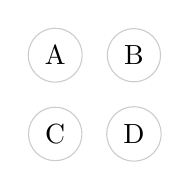
\begin{tikzpicture}
  [scale=.5,auto=left,every node/.style={circle,draw=black!20}]%{circle,border=black!20}]
  \node (v1) at (1,3) {A};
  \node (v2) at (3,3) {B};
  \node (v3) at (1,1) {C};
  \node (v4) at (3,1) {D};
  \end{tikzpicture}

  Conditional independence relationships:\\
  $(A \independent B\ |\ D)$\\
  $(A \independent B\ |\ C,D)$\\
  $(A \independent D\ |\ B,C)$\\
  \end{center}
\end{minipage}  
\begin{minipage}{.25\textwidth}
  \begin{flushleft} Stage I:
  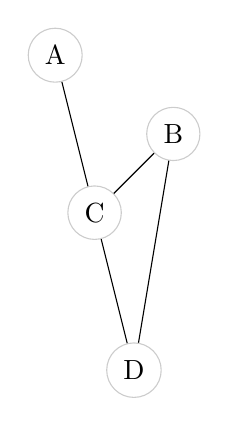
\begin{tikzpicture}
  [scale=.5,auto=left,every node/.style={circle,draw=black!20}]%{circle,border=black!20}]
  \node (v1) at (1,11) {A};
  \node (v2) at (4,9) {B};
  \node (v3) at (2,7) {C};
  \node (v4) at (3,3) {D};

  \foreach \from/\to in {v1/v3,v2/v3,v2/v4,v3/v4}
     \draw (\from) -- (\to);
  \end{tikzpicture}\\
  $S_{AB} = \{D\}$\\
  $S_{AD} = \{B,C\}$\\
  no further minimal separating sets found
  \end{flushleft}
\end{minipage}  
\begin{minipage}{.23\textwidth}
  \begin{flushleft} Stage II:
  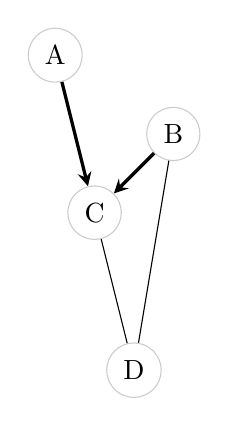
\begin{tikzpicture}
  [scale=.5,auto=left,every node/.style={circle,draw=black!20}]%{circle,border=black!20}]
  \node (v1) at (1,11) {A};
  \node (v2) at (4,9) {B};
  \node (v3) at (2,7) {C};
  \node (v4) at (3,3) {D};

  \foreach \from/\to in {v2/v4,v3/v4}
    \draw (\from) -- (\to);
    
  \begin{scope}[very thick, -stealth]
  \foreach \from/\to in {v1/v3,v2/v3}
    \draw (\from) -> (\to);
  \end{scope}
  \end{tikzpicture}\\
  ACD: $C \in S_{AD}$,\\ no arrows\\
  ACB: $C \notin S_{AB}$,\\ i.e.\ $A \rightarrow C \leftarrow B$
   \end{flushleft}
\end{minipage}  
\begin{minipage}{.23\textwidth}
  \begin{flushleft} Stage III:
  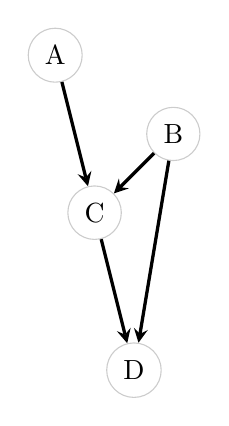
\begin{tikzpicture}
  [scale=.5,auto=left,every node/.style={circle,draw=black!20}]%{circle,border=black!20}]
  \node (v1) at (1,11) {A};
  \node (v2) at (4,9) {B};
  \node (v3) at (2,7) {C};
  \node (v4) at (3,3) {D};
  \begin{scope}[very thick, -stealth]
    \foreach \from/\to in {v1/v3,v2/v3,v2/v4,v3/v4}
    \draw (\from) -> (\to);
  \end{scope}  
 \end{tikzpicture}\\
  $C \rightarrow D$, otherwise new v-structure\\
  $B \rightarrow D$, otherwise directed cycle
   \end{flushleft}
\end{minipage}
\caption{Illustrating the phases of the basic PC algorithm}
\end{figure}

The result computed by the PC algorithm is the minimal graph structure whose d-separation relationships correspond exactly to the conditional independencies in the distribution, i.e. it will contain all those links which we must assume in order to explain the conditional independence properties of the data, and not a single additional link which would not be necessary. A procedure like the PC algorithm therefore implements Occam's razor, the scientific principle which requires us to pick among adequate explanations the one for which we need to make the smallest number of assumptions. The central role of Occam's razor is reflected by the importance of avoiding overfitting in machine learning, where it is typically possible to perfectly model the observable data using a complex model with many parameters (e.g. a fully connected graph), but due to the more difficult inference task, complex models are less likely to classify unseen examples well. It therefore makes sense for inference algorithms to infer the least complex model which still fits the observable data, and this is what the PC algorithm does for joint distributions of causally sufficient sets of variables.

\subsubsection{More recent variants}
The vanilla PC algorithm as I just presented it takes an unnecessary risk in selecting the neighbors out of which separating set candidates are formed. If the distribution is faithful to some DAG, $(A \indep B\ |\ pa(A))$ implies that $A$ and $B$ are independent given a set of nodes lying on undirected paths between $A$ and $B$. Conditioning on variables that are not on any connecting path will not cause any blockage of information flow. Therefore, it suffices to include only nodes on connecting paths in separating set candidates. \citet[5.4.2.3]{spirtes_ea_2000} call this modification the \textit{\isi{PC* algorithm}}, but advise shifting to the more exact separating set candidate selection criterion only after the graph was already thinned out, due to the high memory overload involved in maintaining a list of all connecting paths between any pair of nodes. I will be using a similar idea in \chapref{sec:6}, where the shape of my data allows me to adapt an explicit flow criterion for prefiltering the possible 
separating sets.

A major problem of the vanilla PC algorithm as well as its PC* variant is that the results can vary widely depending on the order in which separating sets are tried out, because the first one will be picked even though there might be many separating sets of the same minimal size. The \textit{Conservative PC} variant\is{Conservative PC algorithm} by \cite{ramsey_ea_2006} differs in not stopping as soon as a single sepset was found, but checking whether the middle variable is present in all or no separating sets of the current size. Unshielded triples where the relevant variable is contained in some, but not all separating sets, are not oriented as colliders, but marked as ambiguous, and prevented from taking part in the propagation rules. This rule will prevent uncertain directionality information from being propagated, but will often leave many edges unoriented.

The \textit{Stable PC} algorithm\is{Stable PC algorithm} by \cite{colombo_maathuis_2014} uses a majority rule to resolve this problem. This variant decides whether to orient each triple as a collider by counting the ratio of all minimal separating sets which contain $B$. Both conservativity and the majority rule remove the order-dependence in the presence of conflicting information, but the PC variants defined in this way still tend to yield either unstable or uninformative results, and must be re-run with different thresholds to detect the stable links.

\subsection{The FCI algorithm}\label{sec:3.2.4}
The FCI algorithm can be seen as a generalization of the PC algorithm to the situation where hidden common causes for some of the observed variables might exist. Such connections will be represented by the bidirected arrows (the edge set $E_\leftrightarrow$) in ancestral graphs.

\subsubsection{Basic version}
The original version of the \textit{FCI (Fast Causal Inference)} algorithm\is{FCI algorithm} was given by \cite{spirtes_ea_2000} as a variant of the PC algorithm in the absence of causal sufficiency. Much as the PC algorithm generates a CPDAG with the goal of approximating the underlying true DAG up to Markov equivalence, the FCI algorithm generates a PAG to represent the Markov equivalence class of the underlying true ancestral graph.

The basic procedure of FCI remains to systematically find separating sets for pairs of observed variables, thinning out a fully connected initial graph until we arrive at a skeleton which only connects pairs of variables that cannot be made independent by conditioning on any combination of the other variables. What makes the FCI algorithm much more complicated than the PC algorithm is that due to the possible existence of latent variables, we cannot assume that we can form a separating set for all pairs of m-separated variables from the neighbors in the current skeleton. To see this, consider the following minimal example taken from \citet[p.129]{spirtes_ea_2000}. We have two pairs of variables $A,B$ and $D,E$, each of which are dependent due to a hidden common cause. The only direct causal influence on $A$ among observed variables is $D \rightarrow A$, and the only influence on $E$ is $B \rightarrow E$. Assume further that neither of the variables $A,B,D,E$ has a direct causal influence on any other 
variable, observed or unobserved, and that there is an additional causal pattern $B \leftarrow F \leftarrow C \rightarrow H \rightarrow D$. This pattern induces a dependence $(A \notindep E)$, but the independence $(A \indep E\ |\ \{B,C,D\})$. There is a separating set which would allow us to delete the link, but this sets includes a variable which is not directly adjacent to either $A$ and $E$ in the true graph.

The question which sets we need to test in order to ensure that a pair of variables $X$ and $Y$ is not m-separated by any subset of the observed variables gives rise to the notion of an \textit{inducing path}. For two disjoint sets $L$ (latent variables) and $S$ (selection variables) of nodes in an ancestral graph which do not contain $X$ or $Y$, an \isi{inducing path} relative to $\langle L,S \rangle$ is a path between $X$ and $Y$ where every intermediate node is either a collider or in $L$, and every collider on the path is either in $S$ or an ancestor of $X$ or $Y$. A crucial result by \cite{richardson_spirtes_2002} shows that $X$ and $Y$ need to be connected in the true ancestral graph (are not m-separated by $Z \cup S$ for any $Z$ disjoint from $L$ and $S$) if and only if there is an inducing path from $X$ to $Y$ relative to $\langle L,S \rangle$.

For the systematic independence tests that are performed to arrive at a skeleton, the original version of the FCI algorithm relied on the notion of an inducing path graph, which, however, turned out \citep{zhang2006} to be less informative than the variant based on ancestral graphs, which is the only one that will be presented here.

After generating an initial skeleton just as in the first phase of the PC algorithm, we cannot yet be sure that all the pairs of still connected variables are actually m-connected in the true ancestral graph, because looking for separating sets only among the neighbors was sufficient to determine d-separation, but does not reliably check for m-separation. Some additional edges might have to be removed, and this is where the inducing path criterion comes in. If we partially orient the links in the initial skeleton by detecting v-structures, many of the paths in the skeleton between each pair of nodes $X$ and $Y$ cannot correspond to inducing paths in the underlying ancestral graph, whereas other might. It therefore suffices to check whether $(X \indep Y\ |\ Z)$ for each combination $Z$ of nodes $Z_k$ connected to $X$ by what might still represent an inducing path. If we manage to break every possible inducing path between the observed variables $X$ and $Y$ in this way, the inducing path criterion allows us to 
remove the link between $X$ and $Y$. In practice, the criterion used to find candidates $Z_k$ in the absence of latent variables checks whether each triple on the path forms either an unshielded collider or a triangle, which is the observable equivalent of an underlying inducing path.

In order to infer the directionality of links in the final skeleton, FCI again relies on the same basic procedure as the PC algorithm, after discarding the directionality information which was used to determine the final skeleton. After redetermining the v-structures as starting points, propagation rules are repeatedly applied, adding partial orientations to additional edges until no further changes occur. The four propagation rules given by \cite{spirtes_ea_2000} have the advantage of still being quite intuitive, but this first version of FCI did not aim to achieve completeness in the sense that it did not necessarily output the most specific maximal ancestral graphs.

\cite{zhang2008} closes this gap by developing and proving the completeness of a rather complex set of orientation rules, giving rise to the \isi{Augmented FCI (AFCI) algorithm}. Since this is the version of the rules which is used in my implementation of RFCI (see below), I will provide each rule here, and give an informal explanation of the intuition behind each of them, as well as their status in the overall inference system. For a compact notation of the conditions under which the rules apply, a star is used as an additional wildcard symbol to represent any arrow end state. This is different from the circle in that the circle represents a concrete state with the potential of being turned into an arrow or a line, whereas the star does not correspond to an actual state, and is only used to keep rule notations compact by matching any possible end symbol.

The first four rules ensure arrowhead completeness, i.e.\ they detect any arrowhead that is present in all members of the Markov equivalence class, based on the assumption that the inferred v-structures are correct. These rules are quite similar to the orientation rules used by the PC algorithm, with one additional rule that looks for discriminating paths which help to distinguish the configurations $A \leftrightarrow B \leftrightarrow C$ and $A \leftrightarrow B \rightarrow C$ in some cases:
\begin{itemize}
 \item $\mathcal{R}1:$ orient unshielded $A \arrowSA B \arrowOS C$ as $A \arrowSA B \rightarrow C$
 \item $\mathcal{R}2:$ orient $A \arrowSO C$ as $A \arrowSA C$ if $A \rightarrow B \arrowSA C$ or $A \arrowSA B \rightarrow C$ 
 \item $\mathcal{R}3:$ orient $D \arrowSO B$ as $D \arrowSA B$ if there is a pair of variables $A$ and $C$ with $(A,C) \notin E$
 which is in configurations $A \arrowSA B \arrowAS C$ and $A \arrowSO D \arrowOA C$
 \item $\mathcal{R}4:$ on a discriminating path $\langle D, \dots, A,B,C \rangle$,
 orient $B \arrowSO C$ as $B \rightarrow C$ if $B$ is in the separating set found for $D$ and $C$,
 and add arrows to form $A \leftrightarrow B \leftrightarrow C$ otherwise
\end{itemize}
Intuitively, the first rule $\mathcal{R}1$ exploits the assumption that in the previous step of the algorithm, we have found exactly the v-structures which are present in the true ancestral graph. This means that we can exclude any arrow that would lead to an additional collider, giving us additional chains. $\mathcal{R}2$ enforces the absence of almost directed cycles in the ancestral graph.

$\mathcal{R}3$ provides a way to infer additional arrows within shielded triples. If in the configuration it acts upon, we added an arrow from $B$ to $D$, the second rule would force us to assume $A \arrowSA D$ in order to avoid a cycle; in the unshielded triple $A \arrowSA D \arrowOS C$, the requirement not to introduce additional v-structures would force an additional arrow $D \rightarrow C$, leading to an (almost) directed cycle $B \rightarrow D \rightarrow C \arrowSA B$, which cannot exist. Therefore, the arrow $D \arrowSA B$ is the only option in this configuration. This inference by contradiction cannot be 
emulated by propagation rules.

The intuition behind $\mathcal{R}4$ is that discriminating paths show some of the behavior of unshielded triples, because on a discriminating path from $X$ to $Y$, the colliders are exactly the nodes which do not occur in any m-separating set for $X$ and $Y$, and the non-colliders are the nodes which occur in every such set. This property allows additional inferences of directionality, much in the same vein as the initial detection of v-structures, but in the presence of bidirectional arcs.

The second block of rules serves to infer the existence of line ends, i.e.\ they are
the overall system's way of detecting selection bias (undirected edges). If we can safely assume that no selection bias is present, these rules will never apply, and can thus safely be ignored:
\begin{itemize}
 \item $\mathcal{R}5:$ orient $A \arrowOO B$ 
 and all edges on an uncovered circle path $\langle A,C,\dots,D,B\rangle$
 where $(A,D) \notin E$ as well as $(B,C) \notin E$ as undirected (\arrowLL), if such a path exists
 \item $\mathcal{R}6:$ orient $B \arrowOS C$  as $B \arrowLS C$ if there is an $A$ with $A \arrowLL B$
 \item $\mathcal{R}7:$ orient $B \arrowOS C$  as $B \arrowLS C$ if there is an $A$ with $A \arrowLO B$, and $(A,C) \notin E$
\end{itemize}
A path is called \textit{uncovered} if every subsequence of length 3 on it forms an unshielded triple, i.e.\ every node is fixed as being either a collider or a non-collider. $\mathcal{R}5$ looks for cycles consisting of unshielded triples, none of which was found to be a v-structure. If we started adding arrows in either direction, $\mathcal{R}1$ would force us to continue adding arrows in the same direction until we arrive at a directed cycle, violating the ancestral graph conditions. Therefore, the only option in such a configuration are undirected links along the entire cycle. $\mathcal{R}6$ directly enforces the ancestral graph property that no arrowhead may point into an undirected edge. The purpose of $\mathcal{R}7$ is similar to $\mathcal{R}3$ in that it covers a reasoning pattern by contradiction that could not be covered by greedy propagation. The reasoning is as follows: If contrary to the rule we assumed $B \arrowAS C$, this would lead to a new v-structure unless $A \arrowLL B$, in which case we 
would again violate the ancestral graph conditions.
 
The third block of rules allows us to turn many partially directed edges $\arrowOA$ into
directed ones, and are therefore essential for the algorithm's ability to distinguish
bidirected from directed arcs in the ancestral graph. Two of these rules rely on finding
paths that are potentially directed, i.e.\ contain only links of the shapes
$\rightarrow$, $\arrowOA$, and $\arrowOO$ (with arrows in the direction of the path):
\begin{itemize}
 \item $\mathcal{R}8:$ orient $A \arrowOA C$ as $A \rightarrow C$ if $A \rightarrow B \rightarrow C$
 or $A \arrowLO B \rightarrow C$
 \item $\mathcal{R}9:$ orient $A \arrowOA C$ as $A \rightarrow C$ if there is an
 uncovered potentially directed path from $A$ to $C$ whose second element $B \neq C$ is not adjacent to $C$
 \item $\mathcal{R}10:$ orient $A \arrowOA C$ as $A \rightarrow C$ if there is a pattern $B \rightarrow C \leftarrow D$,
 and two uncovered potentially directed paths from $A$ to $B$ and from $A$ to $D$, the second elements of which
 (possibly $B$ or $D$) do not coincide, and are not adjacent
\end{itemize}
The rule $\mathcal{R}8$ is again a rule which enforces the non-existence of directed cycles, exploiting the additional conditions imposed on a mixed graph. More specifically, this rule prevents the situation where an arrowhead points into an undirected edge, a condition which was not enforced by $\mathcal{R}2$. The role of $\mathcal{R}9$ is very much analogous to $\mathcal{R}5$, in that it looks for and prevents configurations which would propagate into an almost directed cycle. $\mathcal{R}10$ encodes another instance of reasoning by contradiction. We know that the two potentially directed paths leading away from $A$ form an unshielded non-collider pattern in $A$ (as a collider would have been detected earlier), which implies that the edge from $A$ into at least one of the paths is directed. If we had $A \arrowAA C$ instead of $A \rightarrow C$, this initial directed link would propagate by $\mathcal{R}1$ along the entire path, leading to an almost directed cycle via $B \rightarrow C \leftarrow D$ and $A \rightarrow C$.

\largerpage[-1]
While the soundness of these propagation rules is comparatively easy to see given the explanations, their joint completeness in the sense that iterative application of these rules will lead to a maximally informative partial ancestral graph is highly non-trivial to prove, and requires large amounts of additional formal machinery. For details on these matters, the reader is referred to the theorems in, and especially the proofs in the appendix of, \cite{zhang2008}.

\subsubsection{More recent variants}
The RFCI (Really Fast Causal Inference) algorithm\is{RFCI algorithm} by \cite{colombo_ea_2012} reconsiders the necessity of the large number of conditional independence tests which typically need to be performed by the FCI algorithm, and manages to reduce the number and order of conditional independence tests by exploiting some additional properties of ancestral graphs. These changes make causal inference without causal sufficiency feasible for dozens of variables, and also make it more stable for small sample sizes, because tests of lower order have more statistical power.


\largerpage[-1]
Where FCI tested all subsets of a set of possible m-separators to arrive at the final skeleton, often leading to a combinatorial explosion of tests which needed to be performed especially in sparse graphs, RFCI confines itself to testing only very few sets beyond immediate neighbors, motivated by some important results. For ease of exposition, I will ignore the existence of a set of selection variables $S$ in the original statements, because I will always have $S = \{\}$, equivalent to absence of selecton bias, in my application.

As the first important result, the unshielded triple rule states that a minimal separating set $Z$ for $X_i$ and $X_k$ contains exactly those ancestors $X_j$ of $X_i$ or $X_k$ where both pairs $X_i$ and $X_j$ and $X_j$ and $X_k$ remain dependent given $Z\backslash\{X_j\}$. The RFCI algorithm exploits this by checking all unshielded triples $\langle X_i, X_j, X_k \rangle$ for violations of this pattern, which are then repaired by finding a new minimal separation set for the link ($X_i \arrowLL X_j$ or $X_j \arrowLL X_k$) that was found to be inadequate, and removing the offending link, possibly removing or creating new unshielded triples.

Secondly, the discriminating path rule states that if a path $\langle X_i, \dots, X_l, X_j, X_k \rangle$ is a discriminating path, and no pair of successive vertices on the path can be made independent by conditioning on any subset of the separating set $S_{X_iX_k}$, then if $X_j \in S_{X_iX_k}$, it is an ancestor and not a descendant of $X_k$, and otherwise it is an ancestor of neither $X_l$ or $X_k$, nor a descendant of $X_k$. This fact is used by the RFCI algorithm on triangles of the form $X_k \arrowAL X_l \arrowAS X_j \arrowOS X_k$, where on a minimal discriminating path $\langle X_i, \dots, X_l, X_j, X_k \rangle$, any edge between pairs of successive vertices violating the rule can be removed. These two rules replace the more straightforward check against all sets of vertices reachable by inducing paths given by the standard FCI algorithm, and manage to lead to many of the edge deletions performed by the refinement stage.

A slight decline in output informativity does persist, however, and can be expressed most concisely as a difference in conditions fulfilled by the PAGs returned by FCI and the ones returned by RFCI. In both variants, absence of an arc between $X_1$ and $X_2$ implies the existence of some separating set $Y$ such that $(X_i \indep X_j\ |\ Y)$, an arrowhead at $X_2$ expresses that $X_2$ is not an ancestor to $X_1$ in any MAG of the equivalence class, and a tail at $X_2$ that $X_2$ is an ancestor to $X_1$ in every such MAG. The difference is in the interpretation of edge existence. In the output of FCI, the existence of an edge between $X_1$ and $X_2$ implies that not a single combination of other nodes in the graph constitutes a separating set for $X_1$ and $X_2$, whereas in the output of RFCI, this guarantee only extends to separating sets built from adjacents of one of the two nodes. An RFCI-PAG might therefore have some spurious additional edges in comparison to the FCI-PAG, which means that it must be 
interpreted in a more cautious way.

The resulting PAG is less informative than the output of FCI in some situations, but as \cite{colombo_ea_2012} show, all the causal information it returns is asymptotically correct (i.e.\ guaranteed to become correct given sufficient amounts of data), and the output provably coincides with the output of FCI on a large class of ancestral graphs. The definition of this class mirrors the difference in edge semantics. The only situation where the RFCI-PAG can have an edge $X_i \arrowSS X_j$ in addition to the FCI-PAG is when there is an inducing path from $X_i$ to $X_j$ relative to the remaining adjacents of $X_i$ as well as another inducing path from $X_j$ to $X_i$ relative to the remaining adjacents of $X_j$ in the initial skeleton, but either there is no inducing path from $X_i$ to $X_j$ relative to the possible d-separation nodes for $X_i$, or no inducing path from $X_j$ to $X_i$ relative to the possible d-separation nodes for $X_j$ in the refined skeleton of FCI. What this rather involved condition boils 
down to is that the superfluous edges can only occur between variables that are not connected by ancestry, and will not have line ends in the output of RFCI (i.e.\ they will not be fully directed).

\largerpage
Since the RFCI algorithm appears to be alone in being able to infer PAGs for dozens of variables without running into severe combinatorial problems, it is the only existing algorithm which is directly applicable to the problem of contact lexical flow inference. I will therefore use my own Java implementation of RFCI to represent the state of the art in causal inference in the absence of causal sufficiency.

\subsection{Alternative algorithms}\label{sec:3.2.5}
While the PC algorithm and its derivatives are mathematically well-motivated and rest on firm theoretical grounds, in practice they suffer from severe error propagation issues if but a single conditional independence test yields an incorrect result. They are thus very unstable, a problem which can become so severe that it is typically necessary to re-run these algorithms with different threshold values for the conditional independence tests, on different variable orderings, and under addition of some random noise, then aggregating the results of the runs into a more stable picture.

However, as we will see in this section, there are good reasons to still focus on constrained-based causal inference for lexical flow inference. To start with, most algorithms in the vast landscape of existing approaches only work on continuous variables, or even only on variables that can be assumed to be normally distributed. Limiting the discussion to approaches which might be relevant for my application, I will only discuss two methods which could in principle be applied to the discrete case, but which I am not exploring any further in this book.

The most important alternative to the constraint-based paradigm can be found in the score-based approaches, which directly model the fit of candidate graphs $G$ to a data representation $D$ as an optimization problem for a score which can be chosen to favor minimal graphs. Using a hill climber or a more advanced general optimization algorithm, a candidate graph $G$ is iteratively modified slightly to test whether the score is improving, until a local maximum is reached. In addition to the advantage of not making any categorically wrong decisions, scores make it possible to quantify the certainty about the result graph. The most popular score-based approach is Greedy Equivalence Search (GES)\is{GES algorithm} as described by \cite{chickering2002}. The first phase of GES starts with the empty graph and greedily adds the edges which improve the score most, until a maximum is reached. In the second phase, some edges are removed again as long as this further improves the score. The main disadvantage of score-based methods is the requirement of causal sufficiency, making it impossible to treat hidden common causes correctly. Also, the huge search space tends to make these methods intractable if a structure is to be built over more than a handful of variables.

A different class of causal inference algorithms proceeds by modeling some of the imprecision in the conditional independence judgments based on Bayesian principles. These algorithms are much more stable and less error-prone in practice, but do not have the advantage of theoretical guarantees such as proofs of completeness. Recently, \cite{claassen_heskes_2012} have proposed to combine both paradigms in order to arrive at a both theoretically sound and computationally stable inference procedure. In their \isi{BCCD algorithm}, a Bayesian score is assigned to each input statement, quantifying the reliability of each piece of knowledge. By processing the constraints in decreasing order of reliability, the PC algorithm can be guided in such a way that errors due to bad conditional independence judgments happen late during the execution, therefore only causing local errors which are not propagated much further. While the algorithm compares favourably with FCI when unfaithful DAG approximations to MAGs are 
inferred, the evaluation on test sets spanning only five variables indicates that this approach will not scale to many variables either.
